\documentclass{scrartcl}
\usepackage[utf8]{inputenc}
%\usepackage[T1]{fontenc}
\usepackage[a4paper, left=2.5cm, right=2.5cm, top=2.5cm, bottom=4cm]{geometry}
\usepackage[english]{babel}
\usepackage{amsmath, amsthm, amssymb, amstext}
\usepackage{listings}
\usepackage{color}
\usepackage{graphicx}
\usepackage{xparse}
\usepackage{fancyhdr}
\usepackage{algorithmicx}
\usepackage{algpseudocode}
\usepackage{algorithm}
\usepackage{parskip}
\usepackage[table]{xcolor}
\usepackage{tabularx}
\usepackage{enumerate}
\usepackage{enumitem}
\usepackage{float}
%\usepackage{minted}
\usepackage {tikz}
\usetikzlibrary{positioning}
\usepackage{marvosym}

\pagestyle{fancy}


\rhead{{\newcommand\and\\\getauthors}}
\author{Felix Bühler\\2973410 \and Clemens Lieb\\3130838 \and Steffen Wonner\\2862123 \and Fabian Bühler\\2953320}
\lhead{\textbf\gettitle}
\title{\gettitle}
\chead{\getsubtitle}
\subtitle{\getsubtitle}

\addtolength{\headheight}{2\baselineskip}
\renewcommand{\headrulewidth}{0pt}

\newcommand{\gettitle}{Distributed systems I\\Winter Term 2019/20}
\newcommand{\getsubtitle}{G2T1 – Assignment 5 (theoretical part)}
\newcommand{\getauthors}{Felix Bühler \and Clemens Lieb \and Steffen Wonner \and Fabian Bühler}
\setlength{\headheight}{53pt}

\begin{document}
\maketitle

\section*{1 - Two-Phase Locking}
\subsection*{a)}

See figure \ref{fig:1a}

\begin{figure}[!ht]
	\centering
	\begin{tikzpicture}
	    \draw[->] (0, 15) -- (0, 0);
	    \draw[->] (3, 15) -- (3, 0);
	    \draw[->] (6, 15) -- (6, 0);
	    \draw[->] (9, 15) -- (9, 0);
	
	    \foreach \t/\p in {1/0,2/3,3/6,4/9} {
	      \draw node at (\p, 16) {\(T_\t\)};
	    };
	
	    % transaction 4 can just be parallel
	    \node at ( 8, 14.5) {\(rL_4[u]\)};
	    \node at ( 8, 13.5) {\(r_4[u]\)};
	    \node at ( 8, 12.5) {\(rL_4[o]\)};
	    \node at ( 8, 11.5) {\(r_4[o]\)};
	    \node at ( 8, 10.5) {\(wL_4[y]\)};
	    \node at ( 8,  9.5) {\(rU_4[u]\)};
	    \node at ( 8,  8.5) {\(rU_4[o]\)};
	    \node at ( 8,  7.5) {\(w_4[y]\)};
	    \node at ( 8,  6.5) {\(wU_4[y]\)};
	    \node at ( 8,  5.5) {\(c_4\)};
	
	    % transaction 1 does not need to wait
	    \node at (-1, 14.5) {\(rL_1[v]\)};
	    \node at (-1, 13.5) {\(r_1[v]\)};
	    \node at (-1, 12.5) {\(wL_1[v]\)};
	    \node at (-1, 11.5) {\(w_1[v]\)};
	    \node at (-1, 10.5) {\(wL_1[x]\)};
	    \node at (-1,  9.5) {\(rU_1[v]\)};
	    \node at (-1,  8.5) {\(wU_1[v]\)};
	    \node at (-1,  7.5) {\(w_1[x]\)};
	    \node at (-1,  6.5) {\(wU_1[x]\)};
	    \node at (-1,  5.5) {\(a_1\)};
	
	    %transaction 2 needs to wait for wU[x]
	    \node at (2, 14.5) {\(wL_2[z]\)};
	    \node at (2, 13.5) {\(w_2[z]\)};
	    \node at (2,  5.5) {\(rL_2[x]\)};
	    \node at (2,  4.5) {\(wU_2[z]\)};
	    \node at (2,  3.5) {\(r_2[x]\)};
	    \node at (2,  2.5) {\(rU_2[x]\)};
	    \node at (2,  1.5) {\(c_2\)};
	
	    %transaction 3 needs to wait for wU[v]
	    \node at (5, 14.5) {\(rL_3[s]\)};
	    \node at (5, 13.5) {\(r_3[s]\)};
	    \node at (5,  8.5) {\(rL_3[v]\)};
	    \node at (5,  7.5) {\(r_3[v]\)};
	    \node at (5,  6.5) {\(wL_3[s]\)};
	    \node at (5,  5.5) {\(rU_3[v]\)};
	    \node at (5,  4.5) {\(rU_3[s]\)};
	    \node at (5,  3.5) {\(w_3[s]\)};
	    \node at (5,  2.5) {\(wU_3[s]\)};
	    \node at (5,  1.5) {\(c_3\)};
	
	    % draw the event markings in the timelines
	    \foreach \x/\y in {0/14.5,0/13.5,0/12.5,0/11.5,0/10.5,0/9.5,0/8.5,0/7.5,0/6.5,0/5.5,%
	                       3/14.5,3/13.5,3/5.5,3/4.5,3/3.5,3/2.5,3/1.5,%
	                       6/14.5,6/13.5,6/8.5,6/7.5,6/6.5,6/5.5,6/4.5,6/3.5,6/2.5,6/1.5,%
	                       9/14.5,9/13.5,9/12.5,9/11.5,9/10.5,9/9.5,9/8.5,9/7.5,9/6.5,9/5.5} {
	        \draw[-] (\x-.25,\y) -- (\x+.25,\y);
	    };
	\end{tikzpicture}
	\caption{Operation timeline for History \(H_1\) using non-strict two-phase locking}
	\label{fig:1a}
\end{figure}

\subsection*{b)}

The transactions 2 and 3 need to be aborted / rolled back.
This is because the abort of transaction 1 does not happen until after the locks for reading uncommitted data have been acquired, resulting in incorrect reads.
To enforce consistency, the transactions must be aborted when transaction 1 is aborted.

\subsection*{c)}

See figure \ref{fig:1c}

Cascading abort does not happen with strict two phase locking because updated information from one transaction is only available for other transactions to read after the transaction either aborted or committed.

\begin{figure}[!ht]
    \centering
    \begin{tikzpicture}
        \draw[->] (0, 15) -- (0, -2);
        \draw[->] (3, 15) -- (3, -2);
        \draw[->] (6, 15) -- (6, -2);
        \draw[->] (9, 15) -- (9, -2);
    
        \foreach \t/\p in {1/0,2/3,3/6,4/9} {
          \draw node at (\p, 16) {\(T_\t\)};
        };
    
        % transaction 4 can just be parallel
        \node at ( 8, 14.5) {\(rL_4[u]\)};
        \node at ( 8, 13.5) {\(r_4[u]\)};
        \node at ( 8, 12.5) {\(rL_4[o]\)};
        \node at ( 8, 11.5) {\(r_4[o]\)};
        \node at ( 8, 10.5) {\(wL_4[y]\)};
        \node at ( 8,  9.5) {\(w_4[y]\)};
        \node at ( 8,  8.5) {\(c_4\)};
        \node at ( 8,  7.5) {\(rU_4[u]\)};
        \node at ( 8,  6.5) {\(rU_4[o]\)};
        \node at ( 8,  5.5) {\(wU_4[y]\)};
    
        % transaction 1 does not need to wait
        \node at (-1, 14.5) {\(rL_1[v]\)};
        \node at (-1, 13.5) {\(r_1[v]\)};
        \node at (-1, 12.5) {\(wL_1[v]\)};
        \node at (-1, 11.5) {\(w_1[v]\)};
        \node at (-1, 10.5) {\(wL_1[x]\)};
        \node at (-1,  9.5) {\(w_1[x]\)};
        \node at (-1,  8.5) {\(a_1\)};
        \node at (-1,  7.5) {\(rU_1[v]\)};
        \node at (-1,  6.5) {\(wU_1[v]\)};
        \node at (-1,  5.5) {\(wU_1[x]\)};
    
        %transaction 2 needs to wait for wU[x]
        \node at (2, 14.5) {\(wL_2[z]\)};
        \node at (2, 13.5) {\(w_2[z]\)};
        \node at (2,  4.5) {\(rL_2[x]\)};
        \node at (2,  3.5) {\(r_2[x]\)};
        \node at (2,  2.5) {\(c_2\)};
        \node at (2,  1.5) {\(wU_2[z]\)};
        \node at (2,  0.5) {\(rU_2[x]\)};
    
        %transaction 3 needs to wait for wU[v]
        \node at (5, 14.5) {\(rL_3[s]\)};
        \node at (5, 13.5) {\(r_3[s]\)};
        \node at (5,  5.5) {\(rL_3[v]\)};
        \node at (5,  4.5) {\(r_3[v]\)};
        \node at (5,  3.5) {\(wL_3[s]\)};
        \node at (5,  2.5) {\(w_3[s]\)};
        \node at (5,  1.5) {\(c_3\)};
        \node at (5,  0.5) {\(rU_3[s]\)};
        \node at (5,  -0.5) {\(rU_3[v]\)};
        \node at (5,  -1.5) {\(wU_3[s]\)};
    
        % draw the event markings in the timelines
        \foreach \x/\y in {0/14.5,0/13.5,0/12.5,0/11.5,0/10.5,0/9.5,0/8.5,0/7.5,0/6.5,0/5.5,%
                           3/14.5,3/13.5,3/4.5,3/3.5,3/2.5,3/1.5,3/0.5,%
                           6/14.5,6/13.5,6/5.5,6/4.5,6/3.5,6/2.5,6/1.5,6/0.5,6/-0.5,6/-1.5%
                           9/14.5,9/13.5,9/12.5,9/11.5,9/10.5,9/9.5,9/8.5,9/7.5,9/6.5,9/5.5} {
            \draw[-] (\x-.25,\y) -- (\x+.25,\y);
        };
    \end{tikzpicture}
    \caption{Operation timeline for History \(H_1\) using strict two-phase locking}
    \label{fig:1c}
\end{figure}

\newpage~
\newpage
\section*{2 - Two-Phase Commit}
\subsection*{a)}

Shown in figure~\ref{fig:2a}. $ N_2 $ and $ N_4 $ are blocked until the 'COMMIT'-Message is received. $ N_3 $ will try to resend the 'COMMIT'-Message until it receives the 'ACK'-Message.

\begin{figure}[!ht]
	\centering
	\begin{tikzpicture}
	\draw[->] (0, 0) -- (0, -13);
	\draw[->] (3, 0) -- (3, -13);
	\draw[->] (6, 0) -- (6, -13);
	\draw[->] (9, 0) -- (9, -13);
	\draw[->] (12, 0) -- (12, -13);
	
	\foreach \t/\p in {1/0,2/3,3/6,4/9,5/12} {
		\draw node at (\p, 1) {\(N_\t\)};
	};

	\draw[->] (6, -0.5) -- node[pos=0.75, above] {prepare} (0, -1.5);
	\draw[->] (6, -0.5) -- node[below] {prepare} (3, -1.5);
	\draw[->] (6, -0.5) -- node[below] {prepare} (9, -1.5);
	\draw[->] (6, -0.5) -- node[pos=0.75, above] {prepare} (12, -1.5);
	
	\draw[->] (0, -2) -- node[pos=0.25, below] {yes} (6, -4);
	\draw[->] (3, -2) -- node[above] {yes} (6, -3);
	\draw[->] (9, -2.5) -- node[above] {yes} (6, -3.5);
	\draw[->] (12, -2.5) -- node[pos=0.25, below] {yes} (6, -4.5);
	
	\draw[->] (6, -5.5) -- node[pos=0.75, above] {COMMIT} (0, -6.5);
	\draw[->] (6, -5.5) -- node[below] {COMMIT} (4, -7);
	\draw node at (3.8, -7) {\Lightning};
	\draw[->] (6, -5.5) -- node[below] {COMMIT} (8, -7);
	\draw node at (8.2, -7) {\Lightning};
	\draw[->] (6, -5.5) -- node[pos=0.75, above] {COMMIT} (12, -6.5);
	
	\draw[densely dotted] (-1, -6.75) -- node[pos=0, above] {$ \text{T}_s $} (13, -6.75);
	
	\draw[->] (6, -7.5) -- node[below] {COMMIT} (4, -8.5);
	\draw node at (3.8, -8.5) {\Lightning};
	\draw[->] (6, -7.5) -- node[below] {COMMIT} (8, -8.5);
	\draw node at (8.2, -8.5) {\Lightning};
	
	\draw[densely dotted] (-1, -9) -- node[pos=0, above] {$ \text{T}_e $} (13, -9);
    
    \draw[->] (0, -9.25) -- node[pos=0.25, below] {ACK} (6, -9.75);
    \draw[->] (12, -9.25) -- node[pos=0.25, below] {ACK} (6, -9.75);
	
	\draw[->] (6, -10) -- node[below] {COMMIT} (3, -11);
	\draw[->] (6, -10) -- node[below] {COMMIT} (9, -11);
	
	\draw[->] (3, -11.5) -- node[below] {ACK} (6, -12.5);
	\draw[->] (9, -11.5) -- node[below] {ACK} (6, -12.5);
	
	\draw[line width=0.4mm, blue] (0, -2) -- node[left] {Blocked} (0, -6.5);
	\draw[line width=0.4mm, blue] (3, -2) -- node[pos=0.25, left] {Blocked} (3, -11);
	\draw[line width=0.4mm, blue] (9, -2.5) -- node[pos=0.25, left] {Blocked} (9, -11);
	\draw[line width=0.4mm, blue] (12, -2.5) -- node[left] {Blocked} (12, -6.5);
	\end{tikzpicture}
	\caption{simple termination protocol}
	\label{fig:2a}
\end{figure}

\subsection*{b)}

Shown in figure~\ref{fig:2b}. $ N_1 $ is getting sent a 'DECISION-REQ'-Message to send the 'COMMIT'-Message to $ N_2 $. Same for $ N_5 $ because $ N_4 $ is not reachable.

\begin{figure}[!ht]
	\centering
	\begin{tikzpicture}
	\draw[->] (0, 0) -- (0, -13);
	\draw[->] (3, 0) -- (3, -13);
	\draw[->] (6, 0) -- (6, -13);
	\draw[->] (9, 0) -- (9, -13);
	\draw[->] (12, 0) -- (12, -13);
	
	\foreach \t/\p in {1/0,2/3,3/6,4/9,5/12} {
		\draw node at (\p, 1) {\(N_\t\)};
	};
	
	\draw[->] (6, -0.5) -- node[pos=0.75, above] {prepare} (0, -1.5);
	\draw[->] (6, -0.5) -- node[below] {prepare} (3, -1.5);
	\draw[->] (6, -0.5) -- node[below] {prepare} (9, -1.5);
	\draw[->] (6, -0.5) -- node[pos=0.75, above] {prepare} (12, -1.5);
	
	\draw[->] (0, -2) -- node[pos=0.25, below] {yes} (6, -4);
	\draw[->] (3, -2) -- node[above] {yes} (6, -3);
	\draw[->] (9, -2.5) -- node[above] {yes} (6, -3.5);
	\draw[->] (12, -2.5) -- node[pos=0.25, below] {yes} (6, -4.5);
	
	\draw[->] (6, -5.5) -- node[pos=0.75, above] {COMMIT} (0, -6.5);
	\draw[->] (6, -5.5) -- node[below] {COMMIT} (4, -7);
	\draw node at (3.8, -7) {\Lightning};
	\draw[->] (6, -5.5) -- node[below] {COMMIT} (8, -7);
	\draw node at (8.2, -7) {\Lightning};
	\draw[->] (6, -5.5) -- node[pos=0.75, above] {COMMIT} (12, -6.5);
	
	\draw[densely dotted] (-1, -6.75) -- node[pos=0, above] {$ \text{T}_s $} (13, -6.75);
	
	\draw[->] (3, -7.5) -- node[pos=0.5, above] {DECISION-REQ} (0, -8);
	\draw[->] (9, -7.5) -- node[pos=0.5, above] {DECISION-REQ} (12, -8);
	
	\draw[->] (0, -8.5) -- node[below] {COMMIT} (3, -9);
	\draw[->] (12, -8.5) -- node[below] {COMMIT} (9, -9);
	
	\draw[densely dotted] (-1, -9.5) -- node[pos=0, above] {$ \text{T}_e $} (13, -9.5);
    
    \draw[->] (3, -10) -- node[below] {ACK} (6, -10.5);
    \draw[->] (9, -10) -- node[below] {ACK} (6, -10.5);
    
    \draw[->] (0, -11) -- node[pos=0.25, below] {ACK} (6, -12);
    \draw[->] (12, -11) -- node[pos=0.25, below] {ACK} (6, -12);
	
	\draw[line width=0.4mm, blue] (0, -2) -- node[left] {Blocked} (0, -6.5);
	\draw[line width=0.4mm, blue] (3, -2) -- node[pos=0.25, left] {Blocked} (3, -9);
	\draw[line width=0.4mm, blue] (9, -2.5) -- node[pos=0.25, left] {Blocked} (9, -9);
	\draw[line width=0.4mm, blue] (12, -2.5) -- node[left] {Blocked} (12, -6.5);
	\end{tikzpicture}
	\caption{cooperative termination protocol}
	\label{fig:2b}
\end{figure}
\newpage
\subsection*{c)}

Shown in figure~\ref{fig:2c}.

\begin{figure}[!ht]
	\centering
	\begin{tikzpicture}
	\draw[->] (0, 0) -- (0, -13);
	\draw[->] (3, 0) -- (3, -2.5);
	\draw node at (3, -2.7) {\Lightning};
	\draw[->] (3, -10) -- (3, -13);
	\draw[->] (6, 0) -- (6, -13);
	\draw[->] (9, 0) -- (9, -13);
	\draw[->] (12, 0) -- (12, -13);
	
	\foreach \t/\p in {1/0,2/3,3/6,4/9,5/12} {
		\draw node at (\p, 1) {\(N_\t\)};
	};
	
	\draw[->] (6, -0.5) -- node[pos=0.75, above] {prepare} (0, -1.5);
	\draw[->] (6, -0.5) -- node[below] {prepare} (3, -1.5);
	\draw[->] (6, -0.5) -- node[below] {prepare} (9, -1.5);
	\draw[->] (6, -0.5) -- node[pos=0.75, above] {prepare} (12, -1.5);
	
	\draw[->] (0, -2) -- node[pos=0.25, below] {yes} (6, -4);
	\draw[->] (3, -2) -- node[above] {yes} (6, -3);
	\draw[->] (9, -2.5) -- node[above] {yes} (6, -3.5);
	\draw[->] (12, -2.5) -- node[pos=0.25, below] {yes} (6, -4.5);
	
	\draw[->] (6, -5.5) -- node[pos=0.75, above] {COMMIT} (0, -6.5);
	\draw[->] (6, -5.5) -- node[below] {COMMIT} (4, -7);
	\draw node at (3.8, -7) {\Lightning};
	\draw[->] (6, -5.5) -- node[below] {COMMIT} (8, -7);
	\draw node at (8.2, -7) {\Lightning};
	\draw[->] (6, -5.5) -- node[pos=0.75, above] {COMMIT} (12, -6.5);
	
	\draw[densely dotted] (-1, -6.75) -- node[pos=0, above] {$ \text{T}_s $} (13, -6.75);
	
	%\draw[->] (6, -8) -- node[pos=0.75, above] {DECISION-REQ} (0, -9);
	\draw[->] (9, -7.5) -- node[pos=0.5, above] {DECISION-REQ} (12, -8);
	
	%\draw[->] (0, -9.5) -- node[below] {COMMIT} (2, -10);
	%\draw node at (2.2, -10) {\Lightning};
	\draw[->] (12, -9) -- node[below] {COMMIT} (9, -9.5);
	
	\draw[densely dotted] (-1, -10) -- node[pos=0, above] {$ \text{T}_e $} (13, -10);
    
    \draw[->] (6, -10.25) -- node[below] {COMMIT} (3, -10.75);
    \draw[->] (3, -11) -- node[below] {ACK} (6, -11.5);
    \draw[->] (9, -10.25) -- node[below] {ACK} (6, -10.75);
    
    \draw[->] (0, -11.5) -- node[pos=0.25, below] {ACK} (6, -12.5);
    \draw[->] (12, -11.5) -- node[pos=0.25, below] {ACK} (6, -12.5);
	
	\draw[line width=0.4mm, blue] (0, -2) -- node[left] {Blocked} (0, -6.5);
	\draw[line width=0.4mm, blue] (3, -2) -- node[pos=0.25, left] {Blocked} (3, -2.5);
	\draw[line width=0.4mm, blue] (3, -10) -- node[pos=0.25, left] {Blocked} (3, -10.75);
	\draw[line width=0.4mm, blue] (9, -2.5) -- node[pos=0.25, left] {Blocked} (9, -9.5);
	\draw[line width=0.4mm, blue] (12, -2.5) -- node[left] {Blocked} (12, -6.5);
	\end{tikzpicture}
	\caption{cooperative termination protocol with node failure}
	\label{fig:2c}
\end{figure}

\newpage
\section*{3 - Data Replication}
\subsection*{a)}
q[X$_A$] = 1\\
q[X$_B$] = 1\\
q[X$_C$] = 3\\
q[X$_D$] = 1\\

q$_w$[X] 1: X$_C$, X$_A$ \\
q$_w$[X] 2: X$_C$, X$_B$ \\
q$_w$[X] 3: X$_C$, X$_D$ \\
q$_w$[X] 4: X$_C$, X$_A$, X$_B$ \\
q$_w$[X] 5: X$_C$, X$_A$, X$_D$ \\
q$_w$[X] 6: X$_C$, X$_B$, X$_D$ \\
q$_w$[X] 7: X$_C$, X$_A$, X$_B$, X$_D$\\


q$_r$[X] 1: X$_A$, X$_B$, X$_D$\\
q$_r$[X] 2: X$_C$\\
q$_r$[X] 3: X$_C$, X$_A$\\
q$_r$[X] 4: X$_C$, X$_B$\\
q$_r$[X] 5: X$_C$, X$_D$\\
q$_r$[X] 6: X$_C$, X$_A$, X$_B$\\
q$_r$[X] 7: X$_C$, X$_A$, X$_D$\\
q$_r$[X] 8: X$_C$, X$_B$, X$_D$\\
q$_r$[X] 9: X$_C$, X$_A$, X$_B$, X$_D$\\

\subsection*{b)}
q$_w$[X] = 6\\
q$_w$[x] 1: X$_C$, X$_D$, X$_A$\\
q$_w$[x] 2: X$_C$, X$_D$, X$_B$\\
q$_w$[x] 3: X$_C$, X$_D$, X$_A$, X$_B$\\


\subsection*{c)}
p$_r$(Y) = 1-((1-p$_K$)*(1-p$_L$))-((1-p$_L$)*(1-p$_M$))-((1-p$_M$)*(1-p$_K$))-((1-p$_K$)*(1-p$_L$)*(1-p$_M$))
To be readable a majority of nodes have to be available, which is 2 in this case. That means that 1-p$_r$(Y) is the probability that more than 1 node fails.

\end{document}
